\documentclass[a4paper,12pt]{article}

\usepackage[margin=2cm]{geometry}
\usepackage[utf8]{inputenc}
\usepackage[english]{babel}
\usepackage{textcomp}

\usepackage[font={small,it}]{caption}

\usepackage{graphicx}
\usepackage{epstopdf}
\usepackage{amsmath}
\usepackage{amsfonts}
\usepackage{mathtools}
\usepackage{dsfont}
\usepackage{color}
\usepackage{verbatim}
\usepackage[inline]{enumitem}

\usepackage{tikz}

\usepackage{cite}
\bibliographystyle{apalike}

% \title{}
% \date{}
% \author{}

\begin{document}



\section{Theory of Linear Response in a Nutshell} \label{sec:linear_response}
    \paragraph{Classically} Consider an electron system subject to small external perturbation $V_\text{ext}(\mathbf{r}, t)$. By definition of the \textit{inverse dielectric function} the total potential $V(\mathbf{r}, t)$ is given by
    \begin{equation} \label{eq:cl:potentials_t}
        V(\mathbf{r}, t) 
            = \int\!\! \text{d}^3 r' \!\! \int\limits_{-\infty}^{t}\!\! \text{d} t'\; \varepsilon^{-1}(\mathbf{r}, \mathbf{r'}, t - t') V_\text{ext}(\mathbf{r'}, t')\; .
    \end{equation}
    The upper bound of the integral over $t'$ is $t$ in place of $\infty$ due to causality: the ``effect'' cannot precede the ``cause''. This is equivalent to saying that $\varepsilon^{-1}(\mathbf{r}, \mathbf{r'}, \tau) = 0$ whenever $\tau < 0$. The Fourier transform of $\varepsilon^{-1}(\mathbf{r}, \mathbf{r'}, \tau)$ is
    \begin{equation} \label{eq:cl:inv_dielectric_w}
        \varepsilon^{-1}(\mathbf{r},\mathbf{r'},\omega) = \int\limits_{0}^{\infty} \!\! \text{d}\tau \; e^{i\omega \tau}\,\varepsilon^{-1}(\mathbf{r}, \mathbf{r'}, \tau)\; .
    \end{equation}
    Applying Titchmarsh's theorem to $\varepsilon^{-1}$, we get that $\varepsilon^{-1}(\mathbf{r}, \mathbf{r'}, \omega)$ is the limit $\eta \to 0+$ of $\varepsilon^{-1}(\mathbf{r}, \mathbf{r'}, \omega + i\eta)$ which is holomorphic in the upper complex plane.
    Taking Fourier transform of eq. \eqref{eq:cl:potentials_t}, we obtain\footnote{ %
\begin{equation*}
\begin{aligned}
    V(\mathbf{r}, \omega) 
        &= \int_{-\infty}^{\infty}\!\!\!\! \text{d}t \; e^{i\omega t}\, V(\mathbf{r}, t) \\
        &= \int\!\! \text{d}^3 r' \!\!
           \int_{-\infty}^{\infty}\!\!\!\! \text{d}t 
           \int_{-\infty}^{t}\!\!\!\! \text{d} t' \;
           e^{i\omega t}\, \varepsilon^{-1}(\mathbf{r}, \mathbf{r'}, t - t') V_\text{ext}(\mathbf{r'}, t') \\
        &= \int\!\! \text{d}^3 r' \!\!
           \int_{-\infty}^{\infty}\! \frac{\text{d}\omega'}{2\pi} 
           \int_{-\infty}^{\infty}\!\!\!\! \text{d}t
           \int_{-\infty}^{t}\!\!\!\! \text{d}t' \;
           e^{i\omega t}e^{-i\omega' t'} \varepsilon^{-1}(\mathbf{r}, \mathbf{r'}, t - t') V_\text{ext}(\mathbf{r'}, \omega') \\
        &= \int\!\! \text{d}^3 r' \!\!
           \int_{-\infty}^{\infty}\! \frac{\text{d}\omega'}{2\pi} V_\text{ext}(\mathbf{r'}, \omega')
           \int_{-\infty}^{\infty}\!\!\!\! \text{d}t
           \int_{-\infty}^{t}\!\!\!\! \text{d}t' \;
           e^{i(\omega - \omega')t}e^{i\omega' (t - t')} \, \varepsilon^{-1}(\mathbf{r}, \mathbf{r'}, t - t')  \\
        &= \int\!\! \text{d}^3 r' \!\!
           \int_{-\infty}^{\infty}\! \frac{\text{d}\omega'}{2\pi} \; V_\text{ext}(\mathbf{r'}, \omega')
           \int_{-\infty}^{\infty}\!\!\!\! \text{d}t \, e^{i(\omega - \omega')t}
           \int_{\infty}^{0}\!\! (-\text{d}\tau) \;
           e^{i\omega' \tau} \, \varepsilon^{-1}(\mathbf{r}, \mathbf{r'}, \tau)  \\
        &= \int\!\! \text{d}^3 r' \!\!
           \int_{-\infty}^{\infty} \!\!\!\! \text{d}\omega' \,
           \varepsilon^{-1}(\mathbf{r}, \mathbf{r'}, \omega') V_\text{ext}(\mathbf{r'}, \omega')
           \cdot \frac{1}{2\pi}\int_{-\infty}^{\infty}\!\! \text{d}t \; e^{i(\omega - \omega')t} \\
        &= \int\!\! \text{d}^3 r' \;
           \varepsilon^{-1}(\mathbf{r}, \mathbf{r'}, \omega) V_\text{ext}(\mathbf{r'}, \omega)\; .
\end{aligned}
\end{equation*}
}
    \begin{equation} \label{eq:cl:potentials_w}
        V(\mathbf{r}, \omega) 
            = \int\!\! \text{d}^3 r' \; \varepsilon^{-1}(\mathbf{r}, \mathbf{r'}, \omega) V_\text{ext}(\mathbf{r'}, \omega)\; .
    \end{equation}
    Eqs. \eqref{eq:cl:inv_dielectric_w} and \eqref{eq:cl:potentials_w} may equivalently be formulated as 
    \begin{equation} \label{eq:cl:result_w}
    \begin{aligned}
        V_\text{ext}(\mathbf{r}, \omega) &= \int\!\! \text{d}^3 r' \varepsilon(\mathbf{r}, \mathbf{r'}, \omega) V(\mathbf{r'})\; ,\text{ where} \\
        \varepsilon(\mathbf{r},\mathbf{r'},\omega) &= \lim_{\eta \to 0+} \varepsilon(\mathbf{r}, \mathbf{r'}, \omega + i\eta) = \lim_{\eta \to 0+} \int\limits_{0}^{\infty} \!\! \text{d}\tau \; e^{i (\omega +i\eta) \tau}\,\varepsilon(\mathbf{r}, \mathbf{r'}, \tau)\; .
    \end{aligned}
    \end{equation}

    \paragraph{Quantum Mechanically} Now consider a system of non-interacting electrons described in a single-particle approximation by a Hamiltonian $\hat H_0$. Let $E_i$ denote single-particle energy levels with corresponding eigenstates $| i \rangle$. One-particle density matrix is then
    \begin{equation} \label{eq:qm:rho_0}
        \hat\rho_0 = \sum_i n_i \, | i \rangle\! \langle i|\; , 
    \end{equation}
    where $n_i$ denotes the occupational number at energy $E_i$ which, in equilibrium, is given by the Fermi-Dirac distribution. Electron density operator is $\hat N(\mathbf{r}) = |\mathbf{r}\rangle \! \langle \mathbf{r}|$. Equation of motion reads
    \begin{equation*}
        i\hbar\frac{\text{d}\hat\rho_0}{\text{d}t} = [\hat H_0, \hat\rho_0 ] = 0\; .
    \end{equation*}
    
    Within RPA (Random Phase Approximation) we are interested in the reponse of the system to the perturbation of the form $\hat V e^{-i(\omega + i\eta) t}$ (\textbf{TODO:} explain $\eta$). In the first order approximation, $\hat\rho = \hat\rho_0 + \hat\rho' + \mathcal{O}(\hat V^2)$, where $\hat\rho_0$ is defined by eq. \eqref{eq:qm:rho_0} and $\hat\rho' \propto \hat V$. We thus have
    \begin{equation} \label{eq:qm:time_evolution}
        \left.
        \begin{aligned}
            i\hbar \frac{\text{d}\hat\rho}{\text{d}t} &= i\hbar \frac{\text{d}\hat\rho_0}{\text{d}t} + i\hbar\frac{\text{d}\hat\rho'}{\text{d}t} \\
            [\hat H, \hat\rho] &= [\hat H_0, \hat \rho_0] + [\hat H_0, \hat \rho'] + [\hat V, \hat \rho_0] e^{-i (\omega + i\eta) t} + \mathcal{O}(\hat V^2)
        \end{aligned} \right\} \implies
        i\hbar \frac{\text{d}\hat\rho'}{\text{d}t} = [\hat H_0, \hat \rho'] + [\hat V, \hat \rho_0] e^{-i (\omega + i\eta) t}\; .
    \end{equation}
    Using an ansatz $\hat\rho' = \widetilde G \hat V e^{-i (\omega + i\eta) t}$, where $\widetilde G$ is some time-independent operator, we obtain\footnote{ %
    Calculating matrix elements:
    \begin{equation*}
    \begin{gathered}
        \langle i | i\hbar \frac{\text{d}\hat\rho'}{\text{d}t} | j \rangle = 
            \hbar(\omega + i\eta)\langle i| \hat\rho' | j \rangle\; , \\
        \langle i | [\hat H_0, \hat\rho'] | j \rangle = (E_i - E_j) \langle i| \hat\rho' | j \rangle\; , \\
        \langle i | [\hat V, \hat\rho_0] | j \rangle = (n_j - n_i) \langle i| \hat V | j \rangle\; .
    \end{gathered}
    \end{equation*}
    Eq. \eqref{eq:qm:time_evolution} now reads
    \begin{equation*}
         \langle i| \hat\rho' |j\rangle =
            \frac{(n_i - n_j)\, e^{-i\omega t + \eta t}}{E_i - E_j - \hbar(\omega + i\eta)} \langle i| \hat V |j \rangle \; .
    \end{equation*}
} % end footnote
    \begin{equation*} 
    \begin{aligned}
        \langle i | \widetilde G \hat V | j \rangle 
            &= \frac{n_i - n_j}{E_i - E_j - \hbar(\omega + i\eta)}\langle i | \hat V | j \rangle \\
            &\equiv \langle i | \hat G | j \rangle \, \langle i | \hat V | j \rangle\; ,
    \end{aligned}
    \end{equation*}
    where we have defined a new operator $\hat G$ by 
    \begin{equation} \label{eq:qm:g_function}
        \langle i | \hat G | j \rangle = \frac{n_i - n_j}{E_i - E_j - \hbar(\omega + i\eta)} \; .
    \end{equation}
    We can now calculate the induced electron density $\delta\hat N(t)$:
    \begin{equation} \label{eq:qm:chi_function_t}
    \begin{aligned}
        \langle \mathbf{r} | \delta\hat N(t) | \mathbf{r} \rangle
            &= \operatorname{Tr}(\hat N(\mathbf{r}) \hat\rho) - \operatorname{Tr}(\hat N(\mathbf{r}) \hat\rho_0) = \operatorname{Tr}(\hat N(\mathbf{r})\hat\rho') \\
            &= \sum_{i,j} \langle j|\mathbf{r}\rangle \langle\mathbf{r}| i\rangle \langle i| \widetilde G \hat V | j \rangle e^{-i (\omega + i\eta) t} \\
            &= \sum_{i,j} \langle i | \hat G | j \rangle \langle j|\mathbf{r}\rangle \langle\mathbf{r}| i\rangle \langle i| \hat V | j \rangle e^{-i (\omega + i\eta) t} \; .
    \end{aligned}
    \end{equation}
    The total potential $\hat V$ is the sum of external potential $\hat V_\text{ext}$ and the potential induced by the variation of the charge density, i.e.
    \begin{equation} \label{eq:qm:self_consistency_t}
        \langle \mathbf{r} | \hat V_\text{tot}(t) | \mathbf{r} \rangle
            = \langle \mathbf{r} | \hat V_\text{ext}(t) | \mathbf{r} \rangle + \int\!\! \text{d}^3 r' \; \langle \mathbf{r} | \hat V_\text{Coulomb} | \mathbf{r'} \rangle \langle \mathbf{r'} | \delta\hat N(t) | \mathbf{r'} \rangle \; ,
    \end{equation}
    where $\hat V_\text{Coulomb}$ is the Coulomb interaction potential. We have also used the fact that $\hat V$ is diagonal in position representation. Using eq. \eqref{eq:qm:chi_function_t} we get\footnote{ %
At point $\mathbf{r}$ we have
    \begin{equation*}
    \begin{aligned}
        \langle \mathbf{r}|\hat V_\text{ext}(t) | \mathbf{r} \rangle 
            &= \langle \mathbf{r} | \hat V_\text{tot}(t) | \mathbf{r} \rangle - \int \!\! \text{d}^3 r' \;  \frac{e^2}{\| \mathbf{r} - \mathbf{r'} \|}\, \langle \mathbf{r'} | \delta \hat N(t) | \mathbf{r'} \rangle \\
            &\overset{\eqref{eq:qm:chi_function_t}}{=} \langle \mathbf{r} | \hat V | \mathbf{r} \rangle e^{-i (\omega + i\eta) t}- \int\!\! \text{d}^3 r' \; \frac{e^2}{\| \mathbf{r} - \mathbf{r'} \|} \sum_{i,j} \langle i | \hat G | j \rangle \, e^{-i (\omega + i\eta) t} \, \langle j |\mathbf{r'}\rangle\langle\mathbf{r'} | i \rangle\langle i | \hat V | j \rangle \\
            &= \left( \langle \mathbf{r} | \hat V | \mathbf{r} \rangle - \sum_{i,j} \langle i | \hat G | j \rangle \!\! \int\!\! \text{d}^3 r' \!\! \int\!\! \text{d}^3 r'' \!\! \int\!\! \text{d}^3 r''' \; \frac{e^2}{\| \mathbf{r} - \mathbf{r'} \|} \, \langle j |\mathbf{r'}\rangle\langle\mathbf{r'} | i \rangle \langle i | \mathbf{r''}\rangle \langle \mathbf{r'''} | j \rangle \langle \mathbf{r''} | \hat V | \mathbf{r'''} \rangle \right) e^{-i (\omega + i\eta) t} \\
            &= \left( \langle \mathbf{r} | \hat V | \mathbf{r} \rangle - \sum_{i,j} \langle i | \hat G | j \rangle \!\! \int\!\! \text{d}^3 r' \!\! \int\!\! \text{d}^3 r'' \; \frac{e^2}{\| \mathbf{r} - \mathbf{r'} \|} \, \langle j |\mathbf{r'}\rangle\langle\mathbf{r'} | i \rangle \langle i | \mathbf{r''}\rangle \langle \mathbf{r''} | j \rangle \langle \mathbf{r''} | \hat V | \mathbf{r''} \rangle \right) e^{-i (\omega + i\eta) t} \; .
    \end{aligned}
    \end{equation*}
} % end footnote
    \begin{equation*}
    \begin{aligned}
        \langle \mathbf{r} | \hat V_\text{ext}(t) | \mathbf{r} \rangle &= \int\!\! \text{d}^3 r' \; \langle \mathbf{r} | \hat \varepsilon(t) | \mathbf{r'} \rangle \langle \mathbf{r'} | \hat V | \mathbf{r'} \rangle \; , \text{ where} \\
        \langle \mathbf{r} | \hat \varepsilon(\tau) | \mathbf{r'} \rangle &= \left( \langle \mathbf{r} | \mathbf{r'} \rangle - \sum_{i,j} \langle i | \hat G | j \rangle \int\!\! \text{d}^3 r'' \; \frac{e^2}{\| \mathbf{r} - \mathbf{r''} \|} \, \langle j |\mathbf{r''}\rangle \langle\mathbf{r''} | i \rangle \langle i | \mathbf{r'}\rangle \langle \mathbf{r'} | j \rangle \right) \, e^{-i (\omega + i\eta) \tau}\; .
    \end{aligned}
    \end{equation*}
    Using Titchmarsh's theorem once again, we obtain
    \begin{equation} \label{eq:qm:result_w}
    \begin{aligned}
        \langle \mathbf{r} | \hat V_\text{ext}(\omega) | \mathbf{r} \rangle &= \int\!\! \text{d}^3 r' \; \langle \mathbf{r} | \hat \varepsilon(\omega) | \mathbf{r'} \rangle \langle \mathbf{r'} | \hat V | \mathbf{r'} \rangle \; , \text{ where} \\
        \langle \mathbf{r} | \hat \varepsilon(\omega) | \mathbf{r'} \rangle 
            &= \lim_{\eta \to 0+} \langle \mathbf{r} | \hat\varepsilon(\omega + i\eta) | \mathbf{r'} \rangle = \lim_{\eta \to 0+} \int\limits_{0}^{\infty} \!\! \text{d}\tau \; e^{i (\omega +i\eta) \tau}\,\langle \mathbf{r} | \varepsilon(\tau) | \mathbf{r'} \rangle \\
            &= \langle \mathbf{r} | \mathbf{r'} \rangle - \lim_{\eta \to 0+} \sum_{i,j} \langle i | \hat G | j \rangle \!\! \int\!\! \text{d}^3 r'' \; \frac{e^2}{\| \mathbf{r} - \mathbf{r''} \|} \, \langle j |\mathbf{r''}\rangle \langle\mathbf{r''} | i \rangle \langle i | \mathbf{r'}\rangle \langle \mathbf{r'} | j \rangle \\
            &= \langle \mathbf{r} | \mathbf{r'} \rangle - \int\!\! \text{d}^3 r'' \;  \langle \mathbf{r} | \hat V_\text{Coulomb} | \mathbf{r''} \rangle \langle \mathbf{r''} | \hat\chi(\omega) | \mathbf{r'} \rangle\; , \\
        \langle \mathbf{r''} | \hat\chi(\omega) | \mathbf{r'} \rangle 
            &= \lim_{\eta \to 0+} \sum_{i,j} \langle i | \hat G | j \rangle \langle j |\mathbf{r''}\rangle \langle\mathbf{r''} | i \rangle \langle i | \mathbf{r'}\rangle \langle \mathbf{r'} | j \rangle \; , \\
        \langle \mathbf{r} | \hat V_\text{Coulomb} | \mathbf{r''} \rangle &= \frac{e^2}{\|\mathbf{r} - \mathbf{r''}\|}\; ,
    \end{aligned}
    \end{equation}
    which is the exact equivalent of eq. \eqref{eq:cl:result_w} in the classical description. $\hat\chi$ is called the \textit{polarizability matrix}.

\newpage
\section{Application}
    We now apply the results of sec. \ref{sec:linear_response} to a finite 2D lattice described in the tight binding approximation. We do the calculation in \textit{atomic basis}, i.e. the basis of local site wave functions $|a\rangle$ ($a \in \{0, N-1\}$, where $N$ is the number of sites). The following assumptions are made:
    \begin{itemize}
    \item $\langle a | b \rangle = \delta_{a,b}$,
    \item atomic basis is complete, i.e. $\sum_{a} |a\rangle\! \langle a| = \hat{\mathds{1}}$,
    \item $| a \rangle$'s are localized around the corresponding sites, i.e. $\langle \mathbf{r} | a \rangle \approx \delta(\mathbf{r} - \mathbf{r_a})$, where $\mathbf{r_a}$ is the position of $a$'th site. This is the key to making a step from analytical formulas to numerical calculations.
    \end{itemize}
    These assumptions essentially mean that the step from position representation to atomic basis is performed by $|\mathbf{r}\rangle \to |a\rangle$, $\mathbf{r} \to \mathbf{r_a}$ and $\int\!\text{d}^3 r \to \sum_{a}$. Eq. \eqref{eq:qm:result_w} now reads\footnote{ %
Eq. \eqref{eq:qm:result_w} was written in Gauss system. For the calculations it is, however, easier to use electron-volts. We thus replace $e^2$ by $\frac{e}{4\pi\epsilon_0}$. We also introduce the \textit{self-interaction potential} $V_0$ to prevent degeneracies in $\langle a | \hat V_\text{Coulomb} | a \rangle$.
}
    \begin{equation} \label{eq:appl:result_w}
    \begin{aligned}
        \langle a | \hat V_\text{ext}(\omega) | a \rangle &= \sum_{b} \langle a | \hat \varepsilon(\omega) | b \rangle \langle b | \hat V | b \rangle \; , \text{ where} \\
        \langle a | \hat\varepsilon(\omega) | b \rangle
            &= \langle a | b \rangle - \sum_{c} \langle a | \hat V_\text{Coulomb} | c \rangle \langle c | \hat\chi(\omega) | b \rangle \; , \\
        \langle a | \hat \chi(\omega) | b \rangle 
            &= \lim_{\eta \to 0+} \sum_{i,j} \langle i | \hat G | j \rangle \langle j | a \rangle \langle a | i \rangle \langle i | b \rangle \langle b | j \rangle\; , \\
        \langle a | \hat V_\text{Coulomb} | b \rangle 
            &= \begin{dcases} 
                \frac{1}{4\pi\epsilon_0} \frac{e}{\|\mathbf{r_a} - \mathbf{r_b}\|} & \text{, if } a \neq b, \\
                V_0 & \text{, if } a = b,
                \end{dcases}
    \end{aligned}
    \end{equation}
        \begin{equation*}
    \end{equation*}
    
    The trick that allows the calculations of $\hat\chi(\omega)$ in a reasonable time is to rewrite it in terms of matrices:
    \begin{equation} \label{eq:appl:computing_chi}
    \begin{aligned}
        \langle a | \hat\chi(\omega) | b \rangle 
            &= \overbrace{A(a,b)}^\text{row vector}\!\!\!\!\!\!\!\! \underbrace{\hat G}_\text{square matrix}\!\!\!\!\!\!\!\!\!\!\! \overbrace{A(a,b)^\dagger}^\text{column vector}
            = \overbrace{\Big( \underbrace{{\hat G}^\text{T} A(a,b)^\text{T}}_\text{\texttt{GEMV}} \Big)^\text{T} A(a,b)^\dagger}^\text{\texttt{DOT}} \; ,\text{ where} \\
        G_{i,j} &= \langle i | \hat G | j \rangle \overset{\eqref{eq:qm:g_function}}{=} \frac{n_i - n_j}{E_i - E_j - \hbar(\omega + i\eta)} \; \text{\ \ with }\eta\text{ small}, \text{ and}\\
        A(a,b)_i &= \langle a | i \rangle \langle i | b \rangle = \langle a | i \rangle \langle b | i \rangle^* \; .
    \end{aligned}
    \end{equation}
    The second form of $\langle a | \hat \chi(\omega) | b \rangle$ with a lot of transposes may seem strange, but it is of utmost importance. It allows us to calculate matrix elements of $\hat \chi(\omega)$ using just two \texttt{BLAS} operations: matrix-vector product (\texttt{GEMV}) and dot-product (\texttt{DOT}). It is now straightforward to write a highly parallel implementation of eq. \eqref{eq:appl:computing_chi} and it will not be discussed here any further.

    With eqs. \eqref{eq:appl:result_w} and \eqref{eq:appl:computing_chi} implemented, we can obtain $\hat \varepsilon(\omega)$ for any system, given its tight-binding Hamiltonian $\hat H$ and sites positions $\big\{\mathbf{r_a} |\, a \in \{0,\dots,N-1\}\big\}$. The measurable quantity (\textbf{TODO:} give links to articles about EELS experiments) is the \textit{loss function}\ \  $-\!\operatorname{Im}\left[\langle \mathbf{q} | \hat\varepsilon^{-1}(\omega) | \mathbf{q} \rangle\right]$, where $|\mathbf{q}\rangle$'s denote momentum eigenfunctions. Let $\epsilon_n(\omega)$'s be eigevalues of $\hat\varepsilon(\omega)$ with the corresponding eigenfunctions $|\phi_n(\omega)\rangle$'s. We can now express the loss function as\footnote{ %
    Obviously, if $\epsilon_n(\omega)$ is an eigenvalue of $\hat \varepsilon(\omega)$ with an eigenvector $|\phi_n(\omega)\rangle$, then $1\!/\!\epsilon_n(\omega)$ is an eigenvalue of $\hat \varepsilon^{-1}(\omega)$ with the same eigenvector. We thus have
    \begin{multline*}
    -\operatorname{Im}\left[\langle \mathbf{q} | \hat\varepsilon^{-1}(\omega) | \mathbf{q} \rangle\right] = -\operatorname{Im}\left[ \sum_{n,m} \langle \mathbf{q} | \phi_n \rangle \langle \phi_n | \hat \varepsilon^{-1}(\omega) | \phi_m \rangle \langle \phi_m | \mathbf{q} \rangle \right] \\ = -\operatorname{Im}\left[ \sum_{n} |\langle \mathbf{q} | \phi_n(\omega) \rangle|^2 \frac{1}{\epsilon_n(\omega)} \right] = - \sum_{n} |\langle \mathbf{q} | \phi_n(\omega) \rangle|^2\cdot \operatorname{Im}\left[ \frac{1}{\epsilon_n(\omega)} \right]\; .
    \end{multline*}
} % end footnote
    \begin{equation*}
        -\operatorname{Im}\left[\langle \mathbf{q} | \hat\varepsilon^{-1}(\omega) | \mathbf{q} \rangle\right] = - \sum_{n} |\langle \mathbf{q} | \phi_n(\omega) \rangle|^2\cdot \operatorname{Im}\left[ \frac{1}{\epsilon_n(\omega)} \right]\; .
    \end{equation*}
    Within the tight-binding approximation $\langle \mathbf{q} | \phi_n(\omega) \rangle$ can be calculated as follows
    \begin{equation*}
        \langle \mathbf{q} | \phi_n(\omega) \rangle = \sum_{a} \!\int\!\!\text{d}^3 r \; \langle \mathbf{q} | \mathbf{r} \rangle \langle \mathbf{r} | a \rangle \langle a | \phi_n(\omega) \rangle = \sum_{a} \langle \mathbf{q} | \mathbf{r_a} \rangle \langle a | \phi_n(\omega) \rangle = \frac{1}{(2\pi)^{3/2}} \sum_{a} e^{-i\mathbf{q}\cdot\mathbf{r_a}} \langle a | \phi_n(\omega) \rangle \; .
    \end{equation*}

\newpage
\section{Experiments}
    Let's now apply the aquired tools to examine plasmonic properties of some systems. For this we need a way of visualising the results. We will follow the approach taken in \cite{plasmonic2015}.

    Classically, plasmons are identified by $\varepsilon(\omega) = 0$. In reality, there is also loss due to the parameter $\eta \neq 0$ in eq. \eqref{eq:appl:result_w}. We therefore seek frequencies $\omega$ such that
    \begin{equation} \label{exp:plasmon_def}
        \hat\varepsilon(\omega)|\phi_n(\omega)\rangle = \epsilon_n(\omega) |\phi_n(\omega)\rangle\;,\text{ with }\epsilon_n(\omega) \in \mathbb{C}\setminus\mathbb{R}\text{, i.e. purely imaginary.}
    \end{equation}
    As noted in \cite{andersen2012spatially}, ``when the imaginary part of eigenvalue $\epsilon_n(\omega)$ does not vary too much around the plasmon frequency $\omega'$'', condition \eqref{exp:plasmon_def} is equivalent to the condition that
    \begin{equation*}
        -\operatorname{Im}[\epsilon_n^{-1}(\omega)] \text{ has a local maximum at }\omega'\;.
    \end{equation*}

    This implies that $\epsilon_n(\omega)$ should be a continuous in the neighbourhood of $\omega'$. The problem is to choose $n$. In which of all the eigenvalues are we interested in? And does $n$ vary with $\omega$ or remain constant? The approach taken in \cite{plasmonic2015} is to let $n$ be a function of $\omega$ defined as the index of the eigenvalue with the highest \ $-\operatorname{Im}[ \epsilon_j^{-1}(\omega)]$. We then seek the maxima of \ $-\operatorname{Im}[\epsilon_{n(\omega)}^{-1}(\omega)]$ and call them \textit{plasmon frequencies}. Although it is not obvious whether such an approach is mathematically valid, the fact that \ $-\operatorname{Im}[\epsilon_{n(\omega)}^{-1}(\omega)]$ turns out to be continuous in the calculations seems like a good physical justification.

    Finally, for each $(\omega, n)$ pair, $\operatorname{Re}[\langle \mathbf{r} |\phi_{n(\omega)}(\omega) \rangle]$ gives a good insight in how the plasmon modes ``look like''. We now discuss a couple of systems for which we've performed the outlined calculations.
 

    \begin{figure}[h] 
    \center
    % GNUPLOT: LaTeX picture with Postscript
\begingroup
  \makeatletter
  \providecommand\color[2][]{%
    \GenericError{(gnuplot) \space\space\space\@spaces}{%
      Package color not loaded in conjunction with
      terminal option `colourtext'%
    }{See the gnuplot documentation for explanation.%
    }{Either use 'blacktext' in gnuplot or load the package
      color.sty in LaTeX.}%
    \renewcommand\color[2][]{}%
  }%
  \providecommand\includegraphics[2][]{%
    \GenericError{(gnuplot) \space\space\space\@spaces}{%
      Package graphicx or graphics not loaded%
    }{See the gnuplot documentation for explanation.%
    }{The gnuplot epslatex terminal needs graphicx.sty or graphics.sty.}%
    \renewcommand\includegraphics[2][]{}%
  }%
  \providecommand\rotatebox[2]{#2}%
  \@ifundefined{ifGPcolor}{%
    \newif\ifGPcolor
    \GPcolortrue
  }{}%
  \@ifundefined{ifGPblacktext}{%
    \newif\ifGPblacktext
    \GPblacktexttrue
  }{}%
  % define a \g@addto@macro without @ in the name:
  \let\gplgaddtomacro\g@addto@macro
  % define empty templates for all commands taking text:
  \gdef\gplbacktext{}%
  \gdef\gplfronttext{}%
  \makeatother
  \ifGPblacktext
    % no textcolor at all
    \def\colorrgb#1{}%
    \def\colorgray#1{}%
  \else
    % gray or color?
    \ifGPcolor
      \def\colorrgb#1{\color[rgb]{#1}}%
      \def\colorgray#1{\color[gray]{#1}}%
      \expandafter\def\csname LTw\endcsname{\color{white}}%
      \expandafter\def\csname LTb\endcsname{\color{black}}%
      \expandafter\def\csname LTa\endcsname{\color{black}}%
      \expandafter\def\csname LT0\endcsname{\color[rgb]{1,0,0}}%
      \expandafter\def\csname LT1\endcsname{\color[rgb]{0,1,0}}%
      \expandafter\def\csname LT2\endcsname{\color[rgb]{0,0,1}}%
      \expandafter\def\csname LT3\endcsname{\color[rgb]{1,0,1}}%
      \expandafter\def\csname LT4\endcsname{\color[rgb]{0,1,1}}%
      \expandafter\def\csname LT5\endcsname{\color[rgb]{1,1,0}}%
      \expandafter\def\csname LT6\endcsname{\color[rgb]{0,0,0}}%
      \expandafter\def\csname LT7\endcsname{\color[rgb]{1,0.3,0}}%
      \expandafter\def\csname LT8\endcsname{\color[rgb]{0.5,0.5,0.5}}%
    \else
      % gray
      \def\colorrgb#1{\color{black}}%
      \def\colorgray#1{\color[gray]{#1}}%
      \expandafter\def\csname LTw\endcsname{\color{white}}%
      \expandafter\def\csname LTb\endcsname{\color{black}}%
      \expandafter\def\csname LTa\endcsname{\color{black}}%
      \expandafter\def\csname LT0\endcsname{\color{black}}%
      \expandafter\def\csname LT1\endcsname{\color{black}}%
      \expandafter\def\csname LT2\endcsname{\color{black}}%
      \expandafter\def\csname LT3\endcsname{\color{black}}%
      \expandafter\def\csname LT4\endcsname{\color{black}}%
      \expandafter\def\csname LT5\endcsname{\color{black}}%
      \expandafter\def\csname LT6\endcsname{\color{black}}%
      \expandafter\def\csname LT7\endcsname{\color{black}}%
      \expandafter\def\csname LT8\endcsname{\color{black}}%
    \fi
  \fi
  \setlength{\unitlength}{0.0500bp}%
  \begin{picture}(7936.00,5102.00)%
    \gplgaddtomacro\gplbacktext{%
      \csname LTb\endcsname%
      \put(682,902){\makebox(0,0)[r]{\strut{} 0}}%
      \put(682,1440){\makebox(0,0)[r]{\strut{} 4}}%
      \put(682,1978){\makebox(0,0)[r]{\strut{} 8}}%
      \put(682,2516){\makebox(0,0)[r]{\strut{} 12}}%
      \put(682,3054){\makebox(0,0)[r]{\strut{} 16}}%
      \put(682,3592){\makebox(0,0)[r]{\strut{} 20}}%
      \put(682,4130){\makebox(0,0)[r]{\strut{} 24}}%
      \put(1008,484){\makebox(0,0){\strut{} 0}}%
      \put(1530,484){\makebox(0,0){\strut{} 4}}%
      \put(2052,484){\makebox(0,0){\strut{} 8}}%
      \put(2575,484){\makebox(0,0){\strut{} 12}}%
      \put(3097,484){\makebox(0,0){\strut{} 16}}%
      \put(3620,484){\makebox(0,0){\strut{} 20}}%
      \put(4142,484){\makebox(0,0){\strut{} 24}}%
      \put(176,2650){\rotatebox{-270}{\makebox(0,0){\strut{}$y$}}}%
      \put(2705,154){\makebox(0,0){\strut{}$x$}}%
      \put(5514,1171){\makebox(0,0)[l]{\strut{}0th iteration (unit cell)}}%
      \put(5514,1440){\makebox(0,0)[l]{\strut{}1st iteration}}%
      \put(5514,2247){\makebox(0,0)[l]{\strut{}2nd iteration}}%
      \put(2706,4779){\makebox(0,0){\strut{}$\approx 6.4$ nm}}%
    }%
    \gplgaddtomacro\gplfronttext{%
    }%
    \gplbacktext
    \put(0,0){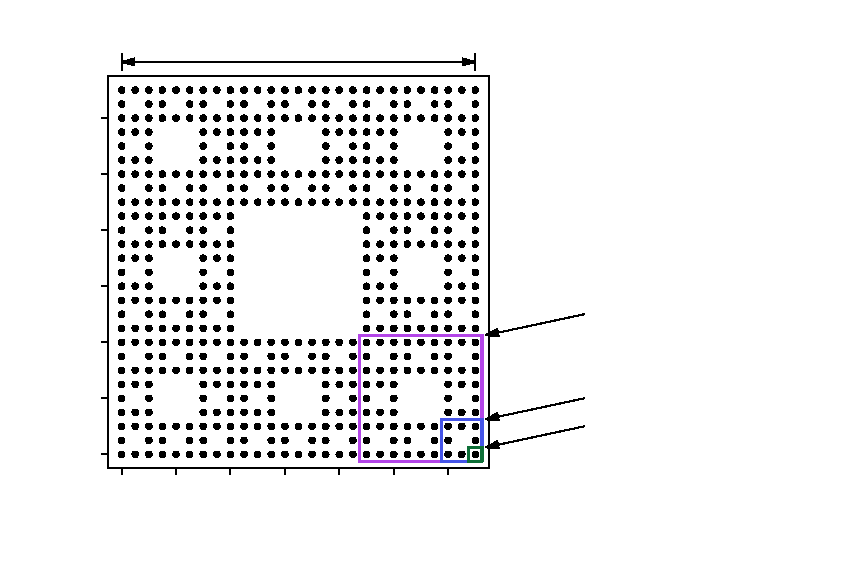
\includegraphics{Coordinates-3rd-SC}}%
    \gplfronttext
  \end{picture}%
\endgroup

    \caption{Third iteration Sierpinski carpet. $x$ and $y$ coordinates are given in terms of lattice constant. Width of the sample is $3^3 = 27$ unit cells. In this case we chose the lattice constant of graphene $a \approx 0.246$ nm, which results in the total width of about six and a half nanometers.}
    \label{fig:coordinates-3rd-SC}
    \end{figure}

\subsection{Third iteration Sierpinski carpet}
    We start by examining a small system --- third iteration Siepinski carpet. The sample is shown in fig. \ref{fig:coordinates-3rd-SC}. Using TIPSI Python package we can construct a tight-binding Hamiltonian for the problem. Hopping value of $2.8$ eV is used. As we need eigenenergies and eigenstates anyway to make use of eq. \eqref{eq:appl:result_w}, we can have a look at the density of states (fig. \ref{fig:dos-3rd-SC}). 
    \begin{figure}[h] 
    \center
    \input{DoS-3rd-SC.tex}
    \caption{Density of states for the 3rd iteration SC. Due to the small size of the system, we can't say much about the distribution of energy eigenvalues. Except that it's highly fluctuating --- as one would expect for a fractal system.}
    \label{fig:dos-3rd-SC}
    \end{figure}
    Although the number of points is quite small (512 atomic sites), we can still extract some information. For example, all possible energies lie within the $(-9.5\text{ eV}, 9.5\text{ eV})$ range. Hence, $E_i - E_j < 19$ eV for any $i, j$. $G_{i,j}$ has $(E_i - E_j - \hbar(\omega + i\eta))$ in the denominator, thus for $\omega$'s greater than $\approx20$ eV, \ $-\operatorname{Im}[ \epsilon_{n(\omega)}^{-1}(\omega)]$ will asymptotically approach zero --- no need to search for plasmons there.

    \begin{figure}[h] 
    \center
    % GNUPLOT: LaTeX picture with Postscript
\begingroup
  \makeatletter
  \providecommand\color[2][]{%
    \GenericError{(gnuplot) \space\space\space\@spaces}{%
      Package color not loaded in conjunction with
      terminal option `colourtext'%
    }{See the gnuplot documentation for explanation.%
    }{Either use 'blacktext' in gnuplot or load the package
      color.sty in LaTeX.}%
    \renewcommand\color[2][]{}%
  }%
  \providecommand\includegraphics[2][]{%
    \GenericError{(gnuplot) \space\space\space\@spaces}{%
      Package graphicx or graphics not loaded%
    }{See the gnuplot documentation for explanation.%
    }{The gnuplot epslatex terminal needs graphicx.sty or graphics.sty.}%
    \renewcommand\includegraphics[2][]{}%
  }%
  \providecommand\rotatebox[2]{#2}%
  \@ifundefined{ifGPcolor}{%
    \newif\ifGPcolor
    \GPcolortrue
  }{}%
  \@ifundefined{ifGPblacktext}{%
    \newif\ifGPblacktext
    \GPblacktexttrue
  }{}%
  % define a \g@addto@macro without @ in the name:
  \let\gplgaddtomacro\g@addto@macro
  % define empty templates for all commands taking text:
  \gdef\gplbacktext{}%
  \gdef\gplfronttext{}%
  \makeatother
  \ifGPblacktext
    % no textcolor at all
    \def\colorrgb#1{}%
    \def\colorgray#1{}%
  \else
    % gray or color?
    \ifGPcolor
      \def\colorrgb#1{\color[rgb]{#1}}%
      \def\colorgray#1{\color[gray]{#1}}%
      \expandafter\def\csname LTw\endcsname{\color{white}}%
      \expandafter\def\csname LTb\endcsname{\color{black}}%
      \expandafter\def\csname LTa\endcsname{\color{black}}%
      \expandafter\def\csname LT0\endcsname{\color[rgb]{1,0,0}}%
      \expandafter\def\csname LT1\endcsname{\color[rgb]{0,1,0}}%
      \expandafter\def\csname LT2\endcsname{\color[rgb]{0,0,1}}%
      \expandafter\def\csname LT3\endcsname{\color[rgb]{1,0,1}}%
      \expandafter\def\csname LT4\endcsname{\color[rgb]{0,1,1}}%
      \expandafter\def\csname LT5\endcsname{\color[rgb]{1,1,0}}%
      \expandafter\def\csname LT6\endcsname{\color[rgb]{0,0,0}}%
      \expandafter\def\csname LT7\endcsname{\color[rgb]{1,0.3,0}}%
      \expandafter\def\csname LT8\endcsname{\color[rgb]{0.5,0.5,0.5}}%
    \else
      % gray
      \def\colorrgb#1{\color{black}}%
      \def\colorgray#1{\color[gray]{#1}}%
      \expandafter\def\csname LTw\endcsname{\color{white}}%
      \expandafter\def\csname LTb\endcsname{\color{black}}%
      \expandafter\def\csname LTa\endcsname{\color{black}}%
      \expandafter\def\csname LT0\endcsname{\color{black}}%
      \expandafter\def\csname LT1\endcsname{\color{black}}%
      \expandafter\def\csname LT2\endcsname{\color{black}}%
      \expandafter\def\csname LT3\endcsname{\color{black}}%
      \expandafter\def\csname LT4\endcsname{\color{black}}%
      \expandafter\def\csname LT5\endcsname{\color{black}}%
      \expandafter\def\csname LT6\endcsname{\color{black}}%
      \expandafter\def\csname LT7\endcsname{\color{black}}%
      \expandafter\def\csname LT8\endcsname{\color{black}}%
    \fi
  \fi
  \setlength{\unitlength}{0.0500bp}%
  \begin{picture}(4534.00,2834.00)%
    \gplgaddtomacro\gplbacktext{%
      \csname LTb\endcsname%
      \put(550,594){\makebox(0,0)[r]{\strut{} 0}}%
      \csname LTb\endcsname%
      \put(550,1055){\makebox(0,0)[r]{\strut{}}}%
      \csname LTb\endcsname%
      \put(550,1516){\makebox(0,0)[r]{\strut{}}}%
      \csname LTb\endcsname%
      \put(550,1977){\makebox(0,0)[r]{\strut{}}}%
      \csname LTb\endcsname%
      \put(550,2437){\makebox(0,0)[r]{\strut{}}}%
      \csname LTb\endcsname%
      \put(958,374){\makebox(0,0){\strut{} 7.2}}%
      \csname LTb\endcsname%
      \put(1442,374){\makebox(0,0){\strut{} 7.3}}%
      \csname LTb\endcsname%
      \put(1926,374){\makebox(0,0){\strut{} 7.4}}%
      \csname LTb\endcsname%
      \put(2409,374){\makebox(0,0){\strut{} 7.5}}%
      \csname LTb\endcsname%
      \put(2893,374){\makebox(0,0){\strut{} 7.6}}%
      \csname LTb\endcsname%
      \put(3377,374){\makebox(0,0){\strut{} 7.7}}%
      \csname LTb\endcsname%
      \put(3861,374){\makebox(0,0){\strut{} 7.8}}%
      \put(176,1581){\rotatebox{-270}{\makebox(0,0){\strut{}\small{$-\operatorname{Im}[\epsilon_{n_1(\omega)}^{-1}(\omega)]$}}}}%
      \put(2409,154){\makebox(0,0){\strut{}\small{$\hbar\omega$, $t$}}}%
    }%
    \gplgaddtomacro\gplfronttext{%
      \csname LTb\endcsname%
      \put(3150,2396){\makebox(0,0)[r]{\strut{}\footnotesize{Fit}}}%
      \csname LTb\endcsname%
      \put(3150,2176){\makebox(0,0)[r]{\strut{}\footnotesize{Numerical}}}%
    }%
    \gplbacktext
    \put(0,0){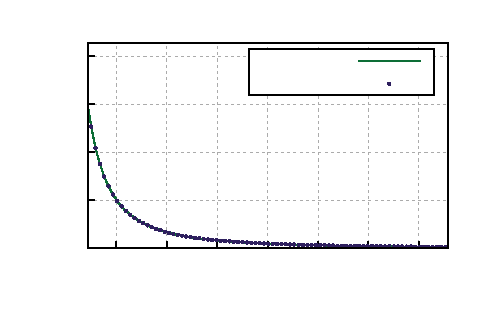
\includegraphics{Spectrum-3rd-SC-Asymptotic}}%
    \gplfronttext
  \end{picture}%
\endgroup

    \caption{This plot shows asymptotic behavior of the loss function at high frequencies. ``Numerical'' denotes the results of the precise numerical calculation. ``Fit'' is obtained by fitting $a / ((b - \omega)^2 + c^2)$ (i.e. eq. \eqref{eq:exp:asymptotic_approx}) to the results of numerical calculations. LSA (Least Square Approximation) gives the following values for the parameters: $a = 1.031 \times 10^{-2}$, $b = 19.779$, $c = 8 \times 10^{-4}$.}
    \label{fig:spectrum-3rd-SC-Asymptotic}
    \end{figure}
    To calculate the dielectric function, we need to choose a couple more parameters of the system. For now, we, again, follow \cite{plasmonic2015} and let the temperature $T$ of the system be $300$ K, chemical potential $\mu = 0.4$ eV, self-interaction coulomb potential $V_0 = 15.78$ eV, and the ``inverse relaxation time'' $\hbar\eta = 0.006$ eV.
    
    Having chosen all configuration parameters we calculate $\hat \varepsilon(\omega)$ for frequencies up to $\approx\! 22$ eV. The two extra eV allow us to look at asymptotic behavior at high frequencies. Let's ignore for a minute the fact that $\hat\epsilon(\omega)$ is a matrix. Using eq. \eqref{eq:appl:result_w} we can approximate the dielectric function by 
    \begin{equation*}
        \epsilon(\omega) \approx 1 - \frac{A}{B - \omega + i\cdot C} \; ,
    \end{equation*}
    and the loss function becomes\footnote{ %
    \begin{equation*}
        \begin{aligned}
        -\operatorname{Im}[\epsilon(\omega)^{-1}] &= -\operatorname{Im}\left[\left(1 - \frac{A}{B - \omega + i\cdot C}\right)^{-1}\right]
        = -\operatorname{Im}\left[\frac{B - \omega + i\cdot C}{B - A - \omega + i\cdot C}\right] \\
        &= -\operatorname{Im}\left[\frac{(B - \omega + i\cdot C)(B - A - \omega - i\cdot C)}{(B - A - \omega)^2 + C^2}\right]
        = -\frac{-C(B - \omega) + C(B - A - \omega)}{(B - A - \omega)^2 + C^2} \\
        &= \frac{CA}{(B - A - \omega)^2 + C^2} \; .
        \end{aligned}
    \end{equation*}
    } % end footnote
    \begin{equation} \label{eq:exp:asymptotic_approx}
        -\operatorname{Im}[\epsilon(\omega)^{-1}] \approx \frac{a}{(b - \omega)^2 + c^2} \;,\text{ where }a=AC ,\;\; b = B-A ,\;\; c = C\;.
    \end{equation}
    Fig. \ref{fig:spectrum-3rd-SC-Asymptotic} shows how good this approximation actually is. This verifies our hypothesis that $\underset{i,j}{\operatorname{max}}|E_i - E_j|$ is a reasonable upper bound for plasmon frequencies.

    \begin{figure}[h] 
    \center
    % GNUPLOT: LaTeX picture with Postscript
\begingroup
  \makeatletter
  \providecommand\color[2][]{%
    \GenericError{(gnuplot) \space\space\space\@spaces}{%
      Package color not loaded in conjunction with
      terminal option `colourtext'%
    }{See the gnuplot documentation for explanation.%
    }{Either use 'blacktext' in gnuplot or load the package
      color.sty in LaTeX.}%
    \renewcommand\color[2][]{}%
  }%
  \providecommand\includegraphics[2][]{%
    \GenericError{(gnuplot) \space\space\space\@spaces}{%
      Package graphicx or graphics not loaded%
    }{See the gnuplot documentation for explanation.%
    }{The gnuplot epslatex terminal needs graphicx.sty or graphics.sty.}%
    \renewcommand\includegraphics[2][]{}%
  }%
  \providecommand\rotatebox[2]{#2}%
  \@ifundefined{ifGPcolor}{%
    \newif\ifGPcolor
    \GPcolortrue
  }{}%
  \@ifundefined{ifGPblacktext}{%
    \newif\ifGPblacktext
    \GPblacktexttrue
  }{}%
  % define a \g@addto@macro without @ in the name:
  \let\gplgaddtomacro\g@addto@macro
  % define empty templates for all commands taking text:
  \gdef\gplbacktext{}%
  \gdef\gplfronttext{}%
  \makeatother
  \ifGPblacktext
    % no textcolor at all
    \def\colorrgb#1{}%
    \def\colorgray#1{}%
  \else
    % gray or color?
    \ifGPcolor
      \def\colorrgb#1{\color[rgb]{#1}}%
      \def\colorgray#1{\color[gray]{#1}}%
      \expandafter\def\csname LTw\endcsname{\color{white}}%
      \expandafter\def\csname LTb\endcsname{\color{black}}%
      \expandafter\def\csname LTa\endcsname{\color{black}}%
      \expandafter\def\csname LT0\endcsname{\color[rgb]{1,0,0}}%
      \expandafter\def\csname LT1\endcsname{\color[rgb]{0,1,0}}%
      \expandafter\def\csname LT2\endcsname{\color[rgb]{0,0,1}}%
      \expandafter\def\csname LT3\endcsname{\color[rgb]{1,0,1}}%
      \expandafter\def\csname LT4\endcsname{\color[rgb]{0,1,1}}%
      \expandafter\def\csname LT5\endcsname{\color[rgb]{1,1,0}}%
      \expandafter\def\csname LT6\endcsname{\color[rgb]{0,0,0}}%
      \expandafter\def\csname LT7\endcsname{\color[rgb]{1,0.3,0}}%
      \expandafter\def\csname LT8\endcsname{\color[rgb]{0.5,0.5,0.5}}%
    \else
      % gray
      \def\colorrgb#1{\color{black}}%
      \def\colorgray#1{\color[gray]{#1}}%
      \expandafter\def\csname LTw\endcsname{\color{white}}%
      \expandafter\def\csname LTb\endcsname{\color{black}}%
      \expandafter\def\csname LTa\endcsname{\color{black}}%
      \expandafter\def\csname LT0\endcsname{\color{black}}%
      \expandafter\def\csname LT1\endcsname{\color{black}}%
      \expandafter\def\csname LT2\endcsname{\color{black}}%
      \expandafter\def\csname LT3\endcsname{\color{black}}%
      \expandafter\def\csname LT4\endcsname{\color{black}}%
      \expandafter\def\csname LT5\endcsname{\color{black}}%
      \expandafter\def\csname LT6\endcsname{\color{black}}%
      \expandafter\def\csname LT7\endcsname{\color{black}}%
      \expandafter\def\csname LT8\endcsname{\color{black}}%
    \fi
  \fi
  \setlength{\unitlength}{0.0500bp}%
  \begin{picture}(9636.00,4534.00)%
    \gplgaddtomacro\gplbacktext{%
      \csname LTb\endcsname%
      \put(814,704){\makebox(0,0)[r]{\strut{} 0}}%
      \csname LTb\endcsname%
      \put(814,1595){\makebox(0,0)[r]{\strut{} 100}}%
      \csname LTb\endcsname%
      \put(814,2486){\makebox(0,0)[r]{\strut{} 200}}%
      \csname LTb\endcsname%
      \put(814,3378){\makebox(0,0)[r]{\strut{} 300}}%
      \csname LTb\endcsname%
      \put(814,4269){\makebox(0,0)[r]{\strut{} 400}}%
      \csname LTb\endcsname%
      \put(946,484){\makebox(0,0){\strut{} 0}}%
      \csname LTb\endcsname%
      \put(2077,484){\makebox(0,0){\strut{} 3}}%
      \csname LTb\endcsname%
      \put(3208,484){\makebox(0,0){\strut{} 6}}%
      \csname LTb\endcsname%
      \put(4339,484){\makebox(0,0){\strut{} 9}}%
      \csname LTb\endcsname%
      \put(5469,484){\makebox(0,0){\strut{} 12}}%
      \csname LTb\endcsname%
      \put(6600,484){\makebox(0,0){\strut{} 15}}%
      \csname LTb\endcsname%
      \put(7731,484){\makebox(0,0){\strut{} 18}}%
      \csname LTb\endcsname%
      \put(8862,484){\makebox(0,0){\strut{} 21}}%
      \put(176,2486){\rotatebox{-270}{\makebox(0,0){\strut{}$-\operatorname{Im}[\epsilon_{n_1(\omega)}^{-1}(\omega)]$}}}%
      \put(5092,154){\makebox(0,0){\strut{}$\hbar\omega$, eV}}%
    }%
    \gplgaddtomacro\gplfronttext{%
    }%
    \gplgaddtomacro\gplbacktext{%
    }%
    \gplgaddtomacro\gplfronttext{%
      \csname LTb\endcsname%
      \put(1907,2026){\makebox(0,0)[r]{\strut{}\footnotesize{0}}}%
      \put(1907,2698){\makebox(0,0)[r]{\strut{}\footnotesize{1}}}%
      \put(1907,3370){\makebox(0,0)[r]{\strut{}\footnotesize{2}}}%
      \put(1907,4042){\makebox(0,0)[r]{\strut{}\footnotesize{3}}}%
      \put(2039,1806){\makebox(0,0){\strut{}\footnotesize{0.4}}}%
      \put(3953,1806){\makebox(0,0){\strut{}\footnotesize{0.5}}}%
      \put(5866,1806){\makebox(0,0){\strut{}\footnotesize{0.6}}}%
    }%
    \gplbacktext
    \put(0,0){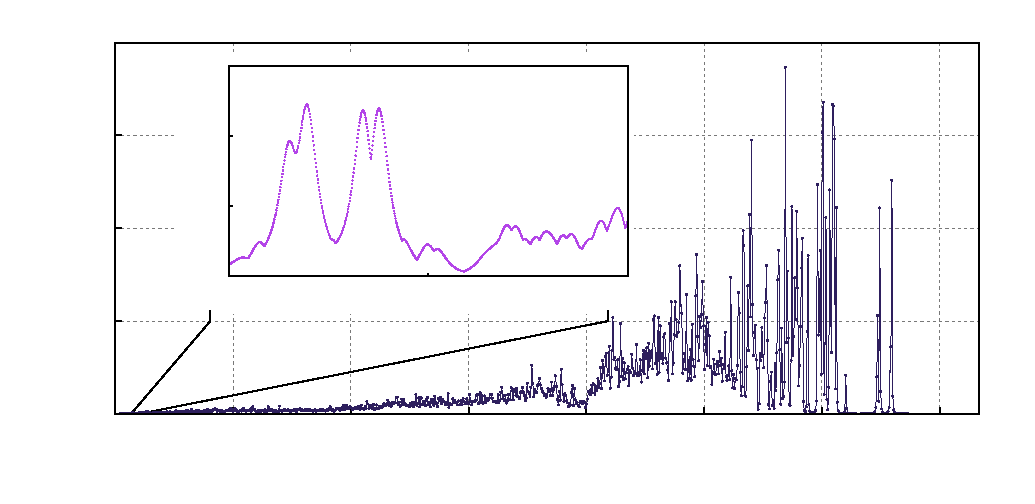
\includegraphics{Spectrum-3rd-SC-Far-Away}}%
    \gplfronttext
  \end{picture}%
\endgroup

    \caption{Loss function spectrum. The spectrum is highly fluctuating (but not self-similar). This makes one wonder whether this spectrum represents actual physical results. Our definition of the loss function may just be ill-formed. Zoomed-in plot shows that this is not the case.}
    \label{fig:spectrum-3rd-SC-far-away}
    \end{figure}

    Spectrum for the full range of frequencies is shown on fig. \ref{fig:spectrum-3rd-SC-far-away}. With our definition of a plasmon high number of sharp peaks means that there are plenty of plasmons. It is interesting to compare the classical definition of plasmon to the condition that loss function has a local maximum. For this we focus on the low-energy part of the spectrum in fig. \ref{fig:spectrum-3rd-SC-far-away} as low-energy plasmon modes are easier to excite experimentally (\textbf{TODO:} this is my intuition, but is it actually true?).



    \begin{figure}[h] 
    \center
    % GNUPLOT: LaTeX picture with Postscript
\begingroup
  \makeatletter
  \providecommand\color[2][]{%
    \GenericError{(gnuplot) \space\space\space\@spaces}{%
      Package color not loaded in conjunction with
      terminal option `colourtext'%
    }{See the gnuplot documentation for explanation.%
    }{Either use 'blacktext' in gnuplot or load the package
      color.sty in LaTeX.}%
    \renewcommand\color[2][]{}%
  }%
  \providecommand\includegraphics[2][]{%
    \GenericError{(gnuplot) \space\space\space\@spaces}{%
      Package graphicx or graphics not loaded%
    }{See the gnuplot documentation for explanation.%
    }{The gnuplot epslatex terminal needs graphicx.sty or graphics.sty.}%
    \renewcommand\includegraphics[2][]{}%
  }%
  \providecommand\rotatebox[2]{#2}%
  \@ifundefined{ifGPcolor}{%
    \newif\ifGPcolor
    \GPcolortrue
  }{}%
  \@ifundefined{ifGPblacktext}{%
    \newif\ifGPblacktext
    \GPblacktexttrue
  }{}%
  % define a \g@addto@macro without @ in the name:
  \let\gplgaddtomacro\g@addto@macro
  % define empty templates for all commands taking text:
  \gdef\gplbacktext{}%
  \gdef\gplfronttext{}%
  \makeatother
  \ifGPblacktext
    % no textcolor at all
    \def\colorrgb#1{}%
    \def\colorgray#1{}%
  \else
    % gray or color?
    \ifGPcolor
      \def\colorrgb#1{\color[rgb]{#1}}%
      \def\colorgray#1{\color[gray]{#1}}%
      \expandafter\def\csname LTw\endcsname{\color{white}}%
      \expandafter\def\csname LTb\endcsname{\color{black}}%
      \expandafter\def\csname LTa\endcsname{\color{black}}%
      \expandafter\def\csname LT0\endcsname{\color[rgb]{1,0,0}}%
      \expandafter\def\csname LT1\endcsname{\color[rgb]{0,1,0}}%
      \expandafter\def\csname LT2\endcsname{\color[rgb]{0,0,1}}%
      \expandafter\def\csname LT3\endcsname{\color[rgb]{1,0,1}}%
      \expandafter\def\csname LT4\endcsname{\color[rgb]{0,1,1}}%
      \expandafter\def\csname LT5\endcsname{\color[rgb]{1,1,0}}%
      \expandafter\def\csname LT6\endcsname{\color[rgb]{0,0,0}}%
      \expandafter\def\csname LT7\endcsname{\color[rgb]{1,0.3,0}}%
      \expandafter\def\csname LT8\endcsname{\color[rgb]{0.5,0.5,0.5}}%
    \else
      % gray
      \def\colorrgb#1{\color{black}}%
      \def\colorgray#1{\color[gray]{#1}}%
      \expandafter\def\csname LTw\endcsname{\color{white}}%
      \expandafter\def\csname LTb\endcsname{\color{black}}%
      \expandafter\def\csname LTa\endcsname{\color{black}}%
      \expandafter\def\csname LT0\endcsname{\color{black}}%
      \expandafter\def\csname LT1\endcsname{\color{black}}%
      \expandafter\def\csname LT2\endcsname{\color{black}}%
      \expandafter\def\csname LT3\endcsname{\color{black}}%
      \expandafter\def\csname LT4\endcsname{\color{black}}%
      \expandafter\def\csname LT5\endcsname{\color{black}}%
      \expandafter\def\csname LT6\endcsname{\color{black}}%
      \expandafter\def\csname LT7\endcsname{\color{black}}%
      \expandafter\def\csname LT8\endcsname{\color{black}}%
    \fi
  \fi
  \setlength{\unitlength}{0.0500bp}%
  \begin{picture}(9636.00,5668.00)%
    \gplgaddtomacro\gplbacktext{%
      \csname LTb\endcsname%
      \put(946,704){\makebox(0,0)[r]{\strut{} 0}}%
      \csname LTb\endcsname%
      \put(946,1644){\makebox(0,0)[r]{\strut{} 0.5}}%
      \csname LTb\endcsname%
      \put(946,2584){\makebox(0,0)[r]{\strut{} 1}}%
      \csname LTb\endcsname%
      \put(946,3523){\makebox(0,0)[r]{\strut{} 1.5}}%
      \csname LTb\endcsname%
      \put(946,4463){\makebox(0,0)[r]{\strut{} 2}}%
      \csname LTb\endcsname%
      \put(946,5403){\makebox(0,0)[r]{\strut{} 2.5}}%
      \csname LTb\endcsname%
      \put(1078,484){\makebox(0,0){\strut{} 0.4}}%
      \csname LTb\endcsname%
      \put(2438,484){\makebox(0,0){\strut{} 0.45}}%
      \csname LTb\endcsname%
      \put(3798,484){\makebox(0,0){\strut{} 0.5}}%
      \csname LTb\endcsname%
      \put(5159,484){\makebox(0,0){\strut{} 0.55}}%
      \csname LTb\endcsname%
      \put(6519,484){\makebox(0,0){\strut{} 0.6}}%
      \csname LTb\endcsname%
      \put(7879,484){\makebox(0,0){\strut{} 0.65}}%
      \csname LTb\endcsname%
      \put(9239,484){\makebox(0,0){\strut{} 0.7}}%
      \put(176,3053){\rotatebox{-270}{\makebox(0,0){\strut{}$-\operatorname{Im}[\epsilon_{n(\omega)}^{-1}(\omega)]$}}}%
      \put(5158,154){\makebox(0,0){\strut{}$\hbar\omega$, eV}}%
    }%
    \gplgaddtomacro\gplfronttext{%
    }%
    \gplbacktext
    \put(0,0){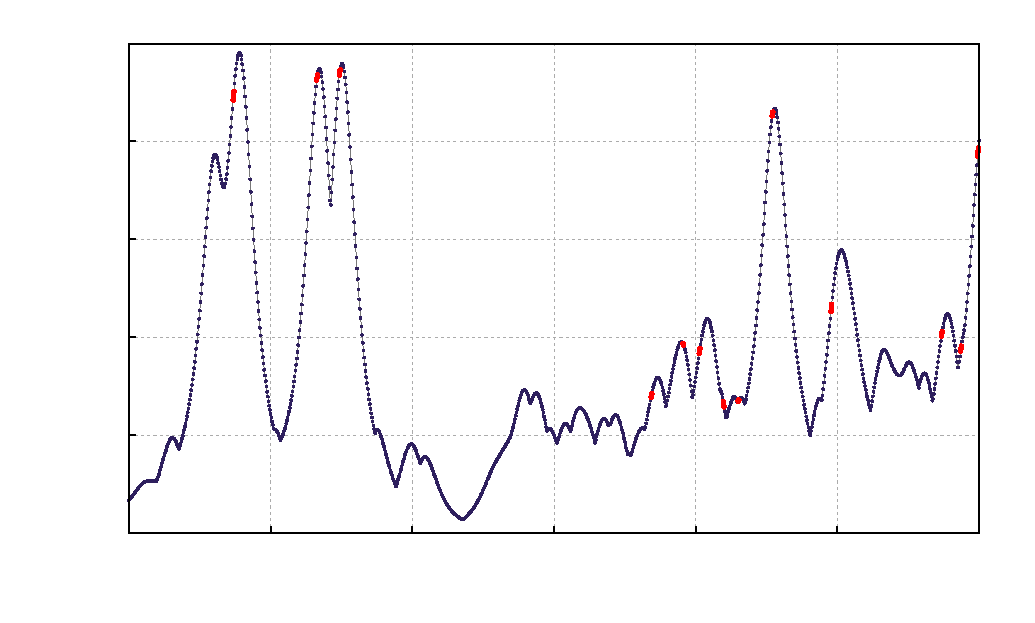
\includegraphics{Spectrum-3rd-SC}}%
    \gplfronttext
  \end{picture}%
\endgroup

    \caption{}
    \label{fig:spectrum-3rd-SC}
    \end{figure}
     


\begin{comment}
    Consider a lattice with $N$ atomic sites where each atom contributes exactly one electron to the valence band. Let $\mathbb{C}^N$ be the Hilbert space of our problem, where $N$ is the number of atomic sites. Here, we assume that each atom contributes exactly one electron to the valence band. $N$: $\operatorname{dim}\,\mathcal{H} = N$. The system is described by a hermitian hamiltonian $H \in \mathcal{B}\left(\mathcal{H}\right)$ with eigenenergies $E_i \in \mathbb{R}$ and eigenstates $|\psi_i\rangle \in \mathcal{H}$ (here, $i \in {0,\dots,N-1}$). 
    
    Within the RPA (Random Phase Approximation) we define the dielectic function as follows. Let electrons in the material be subject to an external perturbation $\hat V_\text{ext} \in \mathcal{B}(\mathcal{H})$ Dielectric function $\hat\varepsilon: \mathbb{R} \to \mathcal{B}\left(\mathcal{H}\right)$ is defined by
    \begin{equation*}
    |\phi_\text{ext}\rangle = \hat\varepsilon(\omega)|\phi_\text{tot}(\omega)\rangle\; ,
    \end{equation*}
    where $\phi_\text{tot}\rangle$ is the total potential in 



    We start with a simple tight-binding approximation where only nearest neighbour hoppings are non-zero. By exact diagonalization of the hamiltonian $\mathcal{H} \in \mathbb{C}^{N \times N}$ eigenenergies $E \in \mathbb{R}^N$ and eigenstates $\psi \in \mathbb{C}^{N \times N}$ are obtained.

    The dielectric function $\varepsilon(\omega) \in \mathbb{C}^{N \times N}$ is then calculated using the following equation
    \begin{equation}
        \varepsilon(\omega)_{a,b} = \mathds{1} - V\cdot\chi(\omega) 
                                  \equiv \mathds{1} - \sum_{n=0}^{N-1} V_{a,n}\chi(\omega)_{n,b}\;,
    \label{eq:dielectric}
    \end{equation}
    where $V \in \mathbb{C}^{N \times N}$ is the Coulomb interaction potential defined as
    \begin{equation}
        V_{a,b} = 
            \begin{dcases} 
                \frac{1}{4\pi\epsilon_0} \frac{e}{\|\mathbf{r_a} - \mathbf{r_b}\|} & \text{, if } a \neq b, \\
                V_0 & \text{, if } a = b,
            \end{dcases}
    \label{eq:coulomb}
    \end{equation}
    and the polarizability matrix $\chi \in \mathbb{C}^{N \times N}$ (as follows from \cite{vonsovskiui1989quantum}) is
    \begin{equation}
        \chi(\omega)_{a,b} = 2\cdot \sum_{i,j\in \{0,\dots,N-1\}}\frac{f_i - f_j}{E_i - E_j - \hbar \left( \omega + i\eta\right)}\psi_{a,i}\psi_{b,i}^*\psi_{b,j}\psi_{a,j}^*.
    \label{eq:polarizability}
    \end{equation}
    Here, $f \in \mathbb{R}^N$ are the occupation numbers that follow from the Fermi-Dirac distribution.

    By calculating $\varepsilon(\omega)$ for a set of frequencies, we obtain the plasmon spectrum, i.e. the loss function as a function of frequency.
\end{comment}


\bibliography{bibliography}
\end{document}
